\chapter{Methods}
\label{cha:Methods}



\section{Task Description}

In this section I will be describing the task and the simulation environment as these two aspects are the foundation of this thesis and will not change over the course of the project.
The task is to develop an agent using reinforcement learning that is able to complete a parcour in a simulated environment without collisions. The agent has to traverse the parcour by passing through a number of goals indicated by pairs of either red or blue blocks without collisions. This problem belongs to the class of single player continuous state and action space problems. At each timestep the agent uses a neural network to process an image from the environment and produce two actions. The two actions are the acceleration values of the left and right wheel, these acceleration values are applied to the wheels until a new action is selected.% The timesteps do not have a fixed duration, a new timestep is started as soon as the last one is finished. The amount of timesteps per minute will be measured? This is like FPS?

The task and agent are simulated using the Unity game engine, the game engine handles the rendering of the environment, collisions, agent movement and reward functions.


\begin{figure}
     \centering
     \subfigure[Example image of the agent at the start of a parcour with 3 goals in Unity]{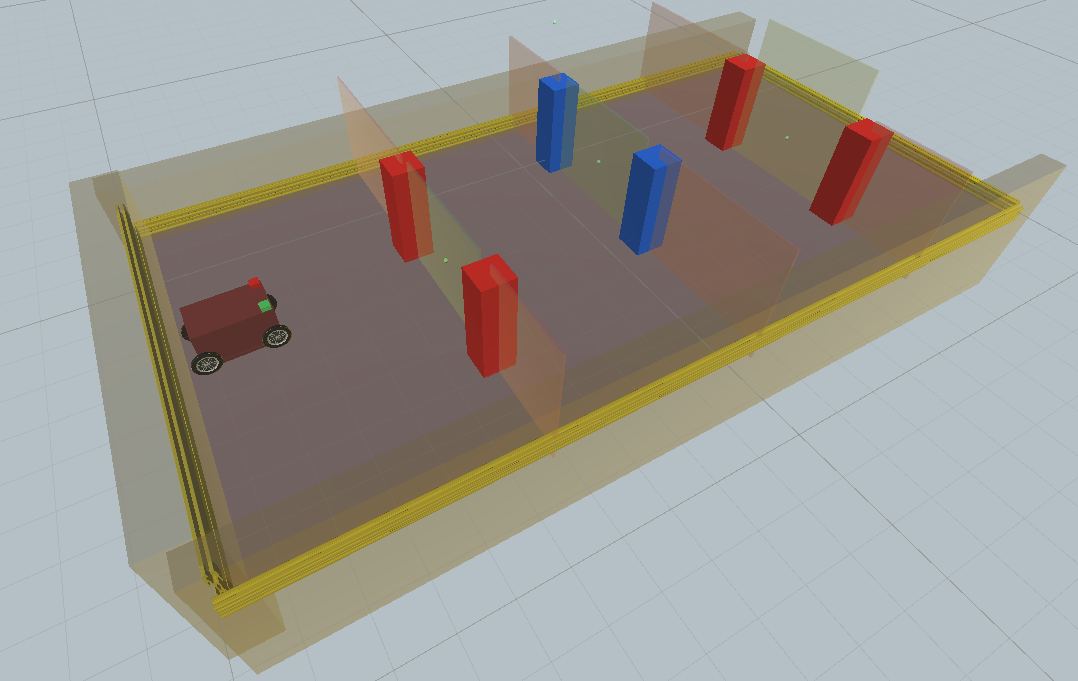
\includegraphics[height=5cm]{Bilder/parcour.png}}\qquad
     \subfigure[Agent camera view]{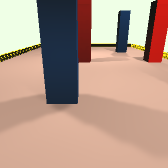
\includegraphics{Bilder/agent_input_image2.png}}\\
     \caption{Unity simulation environment and agent camera view}
\end{figure}


\iffalse
     \begin{figure}[h!]
          \centering
          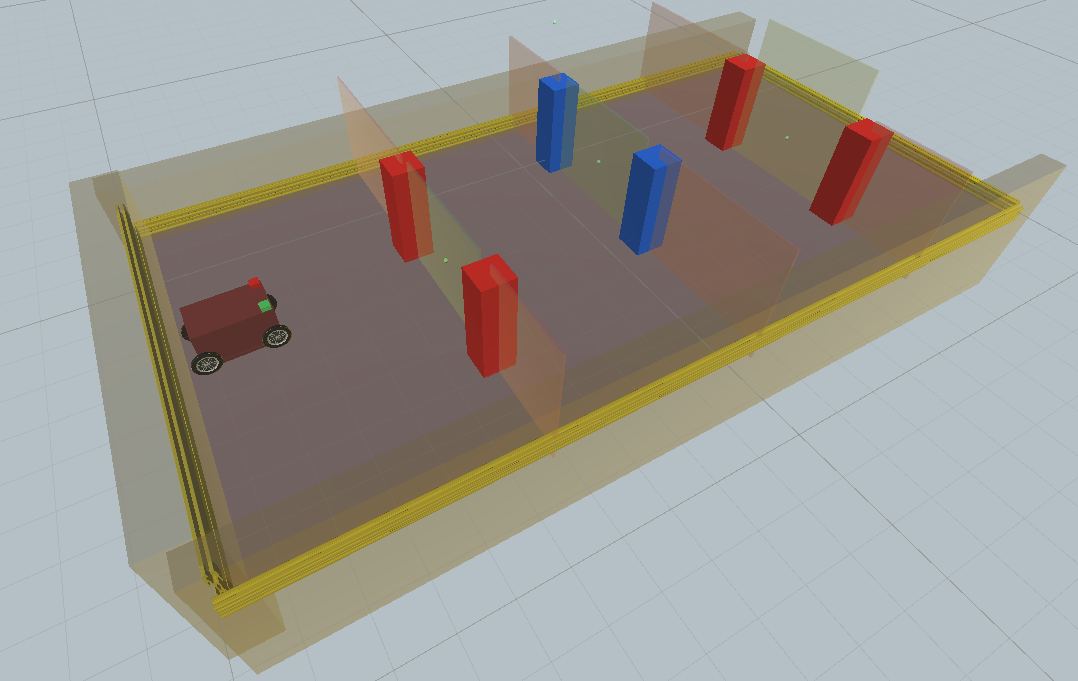
\includegraphics[height=7cm]{Bilder/parcour.png}\\[2.5ex]
          \caption{Example image of the agent at the start of a parcour with 3 goals in Unity}
          \label{task}
     \end{figure}
     \begin{figure}[h!]
          \centering
          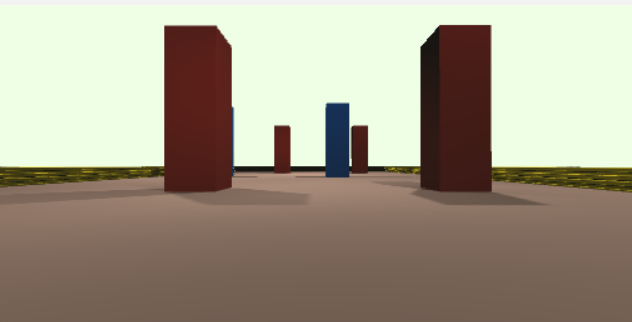
\includegraphics[height=7cm]{Bilder/agent_input_image.png}\\[2.5ex]
          \caption{Example image that will be processed by the agent's convolution neural network.}
          \label{input_image}
     \end{figure}
\fi

% mention the similarity/simplicity of the task


\section{Reinforcement learning algorithm and frameworks}

As outlined in the related works section many different RL algorithms can be used to solve single player continuous state and action space problems. The PPO algorithms is most commonly used for problems of this class and has already been successfully used in the investigated task \autocite{maximilian}. The MuZero \autocite{alphagoimprovementmuzero} could also be used, however this algorithm does require a lot more compute resources during training and inference.
In this thesis the PPO algorithm will be used.

There are multiple approaches to training an agent in the Unity simulation environment as highlighted in the related works section, it is not yet decided which approach will be chosen, therefore I will quickly describe the possible scenarios and highlight their advantages and disavdantages.

\subsection*{Unity and ML-Agents}

Reinforcement learning agents can be trained directly in the Unity simulation environment using the ML-Agents framework \autocite{mlagents}. This approach has the advantage of being very simple to implement and use, since the agent and simulation are in the same framework. The biggest disadvantage of this approach is that it might be difficult to implement some of the implementation details that might be used in this thesis such as the proposed changes for dealing with delayed rewards.
The PPO algorithm by \autocite{mlagents} was used in \autocite{maximilian} to successfully train the agent on the investigated task.

\subsection*{Unity and separate reinforcement learning frameworks}

There are many reinforcement learning frameworks publicly available that can be used to train agents in simulated environments, such as the OpenAI's baselines \autocite{sb3} and Google's dopamine \autocite{dopamine}. These frameworks often support the Gymnasium API \autocite{gymnasium}, wrapping the Unity simulation environment in a Gymnasium environment would allow for easy use of these frameworks. This approach has the advantage of being able to use the many features of these frameworks and makes it easy to change the training algorithms which might be necessary for the investigated implementation details. The disadvantage of this approach is that it might be difficult to wrap the Unity simulation environment in a Gymnasium environment, there already exist frameworks to help with this \autocite{peacefulpie}.


% maybe mention the similarity/simplicity of the task here to show PPO is good


\section{Investigated implementation details}

The goal of this thesis is to answer two questions with a subitem each.
\begin{enumerate}
     \item Is it possible to train an agent to reliably solve the parcours of all difficulty levels?
           \begin{itemize}
                \item Are memory mechanisms necessary in achieving this?
           \end{itemize}
     \item Is it possible to use an end-to-end trained CNN to make the agent robust to changing light conditions?
           \begin{itemize}
                \item Is it possible to use a CNN which is small enough to be used in the JetBot?
           \end{itemize}
\end{enumerate}

\subsection{Improvements for training the agent}

\subsubsection{Reward shaping}

Reward shaping is the practise of providing reinforcement learning agents with frequent and accurate rewards. This helps the agent develop the desired behaviour quicker and more reliably since reward signals are less sparse with reward shaping \autocite{drl_for_ad}. This practice was already employed by \autocite{maximilian} by providing the agent with a reward proportional to its speed, this encourages the agent to drive faster and thus hopefully complete the parcour quicker. This thesis will investigate the use of a reward proportional to the difference in distance to the next goal between timesteps, this should encourage the agent to drive towards the next goal and to drive faster in this direction.


\subsubsection{Dealing with delayed rewards}
Delayed rewards can be a big problem in reinforcement learning and make the training process difficult. Delayed rewards are rewards that are not obtained immediately after the responsible action is taken. In our environment an action \(a_n\) (e.g. turning right) may lead to a collision at state \(s_{n+x}\) which results in a negative reward for action \(a_{n+x}\). The RL algorithm might fail learn to avoid the action \(a_n\).

There are a multiple approaches to dealing with delayed rewards. These approaches use the reward at the current timestep and the near future. These approaches result in a more accurate and dense reward signal and can improve the training stability and performance of the agent.
N-step bootstrapping uses the rewards at the current step and the next \(n\) steps \autocite{nstepbootstrapping}.
A similar approach does not use the reward from the next \(n\) steps but rather the cumulative reward encountered in the next \(n\) seconds \autocite{trackmania}. Due to the continuous nature of the environment this approach might be more suitable than the previous one.


\subsubsection{Time perception}

Two configurations of the agent by \autocite{maximilian} used a memory to enhance the agent's input, the memory consisted of the input of the last few steps of the agent. This technique of stacking the history has been widely used in RL for continuous \autocite{atari} and discrete action spaces \autocite{alphago}. This allows the agent to perceive object movement, time and velocities \autocite{atari}.
In our case the agent needs a history since the next goal could leave the agent's current field of vision.

%However since the investigated environment does not have fixed timesteps this approach might not be as effective. The time elapsed between two steps can vary due to many factors such as varying compute resources. It could prove useful to provide the model with the input of the last few steps and in addition the elapsed time between these steps. % these few sentences only make sense if the varying time is dicussed in the first part of the Methods section

% TODO test other memory mechanisms?
% like for example also feeding the previous time step's hidden layer activation as input
% that way the agent would know the previous "decision" not just the previous input

\subsection{Improvements for Light setting robustness} \label{light_setting_robustness}

\subsubsection{Convolutional Neural Networks}

The works by \autocite{merlin_flach} and \autocite{maximilian} showed that the agent's performance greatly depended on the quality of the input preprocessing pipeline. This object detection pipeline had difficulties detecting objects under varying light settings. This thesis will investigate using convolutional neural networks instead of an object detection pipeline, this should make the agent more robust to varying light settings and improve the performance of the agent.
Using convolutional networks to process images is a common practise in the field of reinforcement learning, due to the ability of these networks to adapt. The convolutional neural network could potentially learn to identify relevant information in images more reliably than the previously used image detection pipeline. The research by \autocite{merlin_flach} showed that not all the information provided by the object detection pipeline was considered to be relevant by the neural network, this could be mitigated by training the CNN end-to-end.
As a starting point for experimentation the CNN architecture will be the same as \autocite{human_level_control}.

% we use the default CnnPolicy network, is it the same as the one described in Atari?
% architecture: https://github.com/DLR-RM/stable-baselines3/blob/d671402c9373391f44d8a2ad11deed615e0f4bae/stable_baselines3/common/torch_layers.py#L89-L106
% it is exactly as described in "Human-level control through deep reinforcement learning"
% \autocite{atari} has a slightly smaller NN

% (more robustness?) (previous input was shit (sim2real paper wegen x, y, width, height input problem)) (previous system higly depended on bounding box detection)


\subsubsection{Feature reduction / preprocessing}

There are several preprocessing approaches that can be used to prepare an image for processing by a convolutional network. The goal of these approaches is to reduce the feature space to increase processing speed, they can also help encourage the network to generalize. The following steps were taken in the foundational \autocite{atari} paper. These techniques will be used due to the similar complexity of our task and many atari games.

\begin{description}
     \item[Downsampling] reduces size of input space
     \item[converting to greyscale] reduces size of input space and potentially removes irrelevant information
     \item[Rescaling pixel values to between 0 and 1] can help the neural network learn quicker % see https://machinelearningmastery.com/how-to-improve-neural-network-stability-and-modeling-performance-with-data-scaling/
\end{description}


\subsubsection{Histogram Equalization}

The previous work this thesis builds upon used the HSV colour space to extract the differently coloured objects. colours in this space consist of three values, one for the hue, saturation and brightness. The hue value was used for extracting the objects. In theory the utilization of this colour space should make the object detection resilient to changes in brightness since this information does not affect the hue value.
Convolutional neural network typically use the RGB colour space or a greyscale colour space. A histogram equalization of the input images could play a big role in making the agent more resilient to changes in illumination, with which the agent by \autocite{maximilian} struggled with. Image d) in \ref{fig:4bildchen} shows the effect of histogram equalization on an image, the image looks worse for identifying objects. This suggests the equalization might not be necessary/useful, it is to be investigated during the implementation/experimentation phase.


%* histogram equalization / enhance contrast (preprocessing) https://stackoverflow.com/questions/39308030/how-do-i-increase-the-contrast-of-an-image-in-python-opencv

% \autocite*{drl_for_ad} shows a lot of best practises in RL for autonomous driving

\begin{figure}
     \centering
     \subfigure[Original Image]{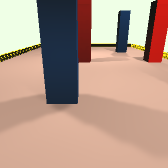
\includegraphics{Bilder/agent_input_image2.png}}\qquad
     \subfigure[Downsampled image]{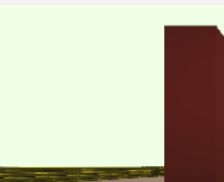
\includegraphics{Bilder/downsampled.png}}\\
     \subfigure[greyscale]{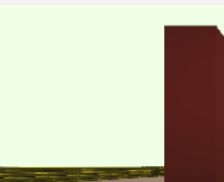
\includegraphics{Bilder/greyscaled.png}}\qquad
     \subfigure[histogram equalized image]{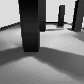
\includegraphics{Bilder/equalized.png}}
     \caption{4 Stages of preprocessing images for the CNN}
     \label{fig:4bildchen}
\end{figure}


\section{Training Process}


\subsection*{Training Parcours}
The PPO Reinforcement Learning algorithm requires the agent to be placed in a simulation environment similar to the evaluation environment to achieve good results. The agent will be placed in an arena with goal objects during training. In previous work \autocite{maximilian} two different training regimes were used, Single-Goal-Training and Full-Map-Training. In Single-Goal-Training the training was stopped after completing the first goal or upon collision. In Full-Map-Training the training was stopped after completing the whole map or upon collision. The reasoning behind Single-Goal-Training is that the agent will encounter a bigger variety of states during training since it will start at different positions in the map. However the Full-Map-Training scenario is closer to the evaluation scenario since the agent has to complete multiple goals in succession during evaluation.
Single-Goal-Training performed worse than Full-Map-Training in the previous work \autocite{maximilian} for all evaluation parcours except for the difficult one.

A third possible regime would be Full-Map-Training with randomized starting positions, this combines both approaches. The Single-Goal-Training is not strictly worse or better than Full-Map-Training. Therefore is not clear what training regime to chose for this thesis, therefore SGT, FMT and FMT with randomized starting positions will be compared during the experimentation phase.
% randomized starting positions also means start at random goals

\subsection*{Training Light Settings}
Since the agent utilizes a Convolutional Neural Network to be resilient towards changing light conditions it is also necessary to train the agent with varying light conditions, otherwise the adaptability of the CNN would not be fully utilized. This way the agent will be able to learn to generalize to different light conditions. The light conditions will be randomized for each training parcour.
Training with fixed light settings could also provide interesting insights when comparing the results to the results of training with varying light settings. If there is enough time the agent will be trained with fixed light settings as well. The comparison would show if the varying light settings during training helps for the generalization to different light settings.

% TODO put a figure with randomized light settings here
% maybe camera image from agents with different light settings

\iffalse
     \begin{figure}
          \centering
          \subfigure[standard lighting]{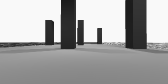
\includegraphics{Bilder/light_setting_pov_standard.png}}\\
          \subfigure[reduced lighting]{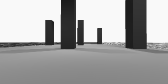
\includegraphics{Bilder/light_setting_pov_reduced_lighting.png}}
          \subfigure[Increased lighting]{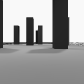
\includegraphics{Bilder/light_setting_pov_increased_lighting.png}}
          \caption{different lightings TODO fix the images currently waiting for Maximilian to tell me how the evaluation environment was configured for different lighting settings}
          \label{fig:3tracks_lighting}
     \end{figure}
\fi

\begin{figure}
     \centering
     \subfigure[Standard Lighting Agent POV]{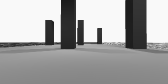
\includegraphics[width=0.25\textwidth]{Bilder/light_setting_pov_standard.png}}\qquad
     \subfigure[Standard Lighting Arena]{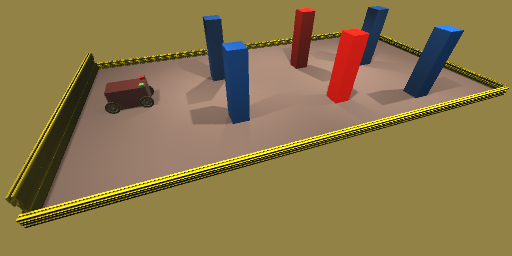
\includegraphics[width=0.5\textwidth]{Bilder/light_setting_arena_standard.png}}
     \subfigure[Reduced Lighting Agent POV]{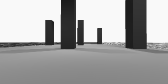
\includegraphics[width=0.25\textwidth]{Bilder/light_setting_pov_reduced_lighting.png}}\qquad
     \subfigure[Reduced Lighting Arena]{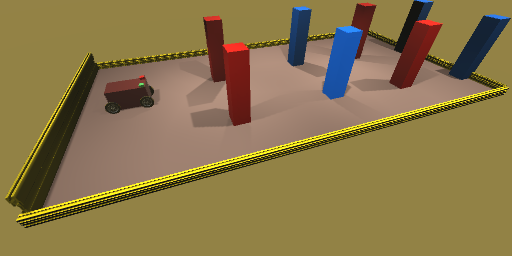
\includegraphics[width=0.5\textwidth]{Bilder/light_setting_arena_reduced_lighting.png}}
     \subfigure[Increased Lighting Agent POV]{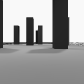
\includegraphics[width=0.25\textwidth]{Bilder/light_setting_pov_increased_lighting.png}}\qquad
     \subfigure[Increased Lighting Arena]{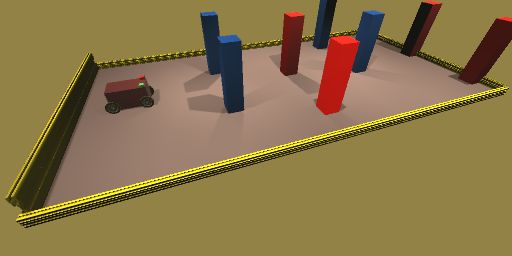
\includegraphics[width=0.5\textwidth]{Bilder/light_setting_arena_increased_lighting.png}}

     \caption{Lighting Agent POV and Arena TODO real images wait for information by Maximilian about how lighting was done} \label{fig:1}
\end{figure}


% TODO do we need an image equalization if the network is trained on varying light conditions?

\subsection*{Data Augmentation}
Convolutional Neural Networks require a lot of data to learn and generalize. Data augmentation is a technique to increase the amount of data available during training by applying transformations to the collected data. Collected data can be used to produce many more training examples by applying transformations such as rotation, translation, scaling, flipping and colour changes. In addition to providing a more diverse set of training data, this saves a lot of time since the new data points are not collected in simulation. \autocite{conditional_imitation_learning} employed a diverse set of data augmentation for their imitation learning approach that used a CNN.
During the training process the collected images will be augmented by applying random transformations to them. The transformations change the image similarly to how different environment conditions (e.g. lighting, camera quality and fog) might change the image. It is not yet decided which transformations will be used, possible candidates are changes in contrast, brightness and tone, as well as filters like Gaussian blur, Gaussian noise, salt-and-pepper noise.
Geometric transformations such as translations and rotations are not used since our control commands are not invariant to these transformations.


\begin{figure}
     \centering
     \subfigure[Original image]{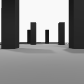
\includegraphics{Bilder/data_entry_original.png}}
     \subfigure[Gaussian Noise Mean 0 Sigma 5]{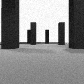
\includegraphics{Bilder/data_entry_augmented_gaussian_sigma_5.png}}
     \subfigure[salt-and-pepper noise]{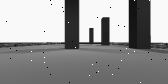
\includegraphics{Bilder/data_entry_augmented_salt_and_pepper.png}}
     \caption{Data augmentation examples}
     \label{fig:data_augmentation}
\end{figure}

% TODO find another paper with data augmentaton
